\chapter{Integrating gene expression data from normal tissues across RNA-Seq studies}%
\label{ch:Transcriptomics}

\vspace*{0.7in}

To pave the way towards
a generalised baseline expression reference for the \emph{normal}
(\ie\ non-disease) human,
I assess in this chapter the similarity
of the tissues sourced from different \Rnaseq\ studies and
the general profiles of their expressed genes.
When I started this project in 2013,
little was known on either the robustness or
the shortcomings and pitfalls of \Rnaseq\ and
its related processing of output data.
Since then, several studies were published assessing \Rnaseq\
robustness (See \Cref{sec:TranssCoop}).
A few are close in scope to my own investigations.
Thus whenever relevant,
I introduce and discuss my results in relation to the published ones.

In the first part of this chapter,
I introduce the working datasets based on the transcriptome studies
(described in \Cref{ch:datasets}).
In a second part,
I appraise the congruence of the interstudy gene expression profiles.
In the third and final part of the chapter,
I dissect the different components that
may contribute the most to (and thus explain)
the overall strong biological correlations that are observed between the studies.

All the work presented in this chapter was performed by myself under the
supervision of \alvis.
I received invaluable advise and help from my discussions with \nuno.
I also received general feedback and comments from \mar, \johan, \sarah, \gos\
and \wolfgang.
\clearpage

\derivativeWork{}
\begin{itemize}[topsep=0pt,nosep]
    \item \fullcite{EBIgxa}
    \item (short talk) Quantitative Genomics 2015 --- Integration of
        independent human RNA-seq datasets: a feasibility study
    \item (poster) ECCB 2014 --- A feasibility study:
        Integration of independent RNAseq datasets
    \item (invited short talk) GM$^2$ 2013 --- Baseline Gene expression Atlas
    \item (flash talk) CSAMA 2013 --- How quantitative is RNA-seq?
\end{itemize}
\clearpage

In the past years,
\Rnaseq\ rapidly gained popularity
for gene expression studies
due to a broader dynamic range than previous technologies
and the promise to enable quantitative profiling \mycite{Marioni2008-xr}.
That technology was an advancement with respect to microarray assays
that are very prone to batch effects and are semiquantitative~\mycite{lee:2006}.
However, \Rnaseq\ studies had shown variation in their conclusions on various
occasions for similar research topics~\mycite{seqcmaqc}.
At the time that I started my \phd,
it appeared that
\Rnaseq\ might share at least partially the problems encountered
with microarray assays.
In fact, \emph{batch effects} restrain the use of direct approaches
for the comparison of independent microarray data,
and the resulting insights are usually limited \mycite{Walsh2015-nf,Rung2013-ul,Lazar2013-lj}.

\section{Working sets}

Through this chapter, I use two working sets
based on subsets of the transcriptomic studies introduced in \Cref{ch:datasets}:
\begin{itemize}[topsep=0pt,nosep]
    \item \setOne: 4 tissues --- 12,268 genes across the 5 \Rnaseq\ studies, and
    \item \setTwo: 23 tissues --- 17,551 genes across 2 of these studies.
\end{itemize}

The following \cref{subsec:transtissueOverlap,subsec:transGeneOverlap}
illustrate the construction of these sets.

While many approaches exist,
I usually consider the most stringent routes,
\ie\ I rather exclude part of the data to infer conclusions than
keep wider datasets and more partial, biased or ambiguous results.
Thus, I identified the identical core of
explored tissues and expressed genes across the studies.
From this base, I created more robust working sets for the meta-analyses.

\subsection{Tissue overlaps across available normal human RNA-Seq studies \quad}%
\label{subsec:transtissueOverlap}
\vspace*{-5mm}
\Cref{fig:VennStudiesT} presents the tissue overlap between the five datasets.
All datasets share at least four tissues:
\heart, \kidney, \liver\ and \testis.
This 4-tissue set is the base of the first working set (\setOne).

The greatest number of shared tissues occurs
between the two most recent studies:
\uhlen~\mycite{Uhlen2015} and \gtex~\mycite{GTExTranscript}.
They constitute the base of a second 23-tissue working set (\setTwo).
This set includes
\Adipose, \Adrenal, \Bladder, \Cortex, \hcolon, \Esophagus,
\Fallopian, \heart, \kidney, \liver, \lung, \Ovary, \Pancreas, \Prostate,
\salivary, \skeletal, \skin, \intestine, \spleen, \stomach, \testis,
\thyroid\ and \uterus.

\begin{figure}[!htbp]
\includegraphics[scale=0.49]{transcriptomics/TransVennTissue.pdf}\centering
\caption[Distribution of unique and shared tissues between the
transcriptomic datasets]
{\label{fig:VennStudiesT}\textbf{Distribution of unique and shared tissues
between the transcriptomic datasets.} The five datasets share four
common tissues: \heart, \kidney, \liver\ and \testis.
The most prominent overlap of tissues (23) is between \uhlen\ and \gtex.
}
\end{figure}
\vspace*{-5mm}

\subsection{Common measured genes for each of the main shared-tissue sets\quad}%
\label{subsec:transGeneOverlap}
\vspace*{-9mm}
As shown in \Crefp{tab:Trans5DF}{},
many of the transcriptomic datasets I use were produced through
polyA-selected library protocols.
Hence,
to avoid unnecessary biases\footnote{See
\Cref{subsec:protcodingOnly}: \nameref{subsec:protcodingOnly}.},
I have limited most of my analyses to \pcgs\ (\ens{76}).
All mitochondrial genes have been filtered out before any \treps{} analysis
(as specified in \Cref{subsec:mito}).

\begin{figure}[!hptb]
    \centering
    \begin{subfigure}[b]{\textwidth}
        \centering \includegraphics[scale=0.6]{transcriptomics/PcodingGenesExpressed1_4tissues.pdf}
        \caption{Four common tissues across the five tissues (\setOne)}\label{fig:ExpGenePcoding1}
    \end{subfigure}

    \begin{subfigure}[b]{\textwidth}
        \centering \includegraphics[scale=0.55]{transcriptomics/vennTissue23_1protcodgenes.pdf}
        \caption{Twenty-three common tissues\\ between Uhlén et al.\
        and GTEx studies (\setTwo)}\label{fig:ExpGenePcoding1_t23}
    \end{subfigure}
    \caption[Unique and shared \pcgs\ expressed (≥1 \FPKM) across RNA-Seq studies]%
    {\textbf{Unique and shared \pcgs\ expressed (≥ 1 \FPKM) across the \Rnaseq\ studies
    for \setOne\ and \setTwo}}
\end{figure}

The Venn diagram presented in \Cref{fig:ExpGenePcoding1} only includes \pcgs\
that are observed\footnote{See
\Cref{sec:ExpressedOrNot}: \nameref{sec:ExpressedOrNot}.}
at least once at 1 \FPKM\ for one of the four shared tissues.
As mentioned in the previous chapter (\Cref{subsec:averagedTissue}~p.~\pageref{def:trep}),
the bulk of expressed genes at this threshold is common
to all five datasets.
While each study presents a tiny portion of genes
that are unique,
overall most genes are detected in at least two studies.
The most considerable contingent of shared gene expression is observed
between \uhlen\ and \gtex.

\Cref{fig:ExpGenePcoding1_t23} presents a similar Venn diagram
which focuses on the set of twenty-three tissues (\setTwo)
between \uhlen\ and \gtex\ studies.
The uniquely expressed genes in each study are negligible compared to the overlap.
They represent less than 0.03\% of the measured genes in each of the studies
(0.026\% for \uhlen; 0.016\% for \gtex).
\begin{comment}
    Gtex:   462/17551 hence 0.02632329\%
    Uhlen:  281/17551 hence 0.01601048\%
\end{comment}

I analysed all the other subgroups of genes
(\ie\ unique to each study or shared only between two to four datasets)
for any functional annotation enrichment.
Neither the \gls{gsea} or the \gls{goa}
provided any conclusive result.

\section{Prevalence of biological signal over technical variabilities at
tissue-level}\label{sec:Trans_ReproExpresTissue}

As I show in \Cref{ch:expression},
the expression levels of biological replicates (\ie\ identical tissue samples)
are highly correlated within the same study
and allow one to group the samples based on their biological source.
Thus, clustering the samples across studies should offer a rough assessment of
the underlying driving forces for the observed gene expression levels.
A clustering by study means that the technical variabilities are stronger
than any biological expression signature
(which is a recurrent observation with microarray studies
due to their stronger batch effects \mycite{Sudmant2015-zt}).
On the other hand,
an interstudy sample clustering by tissue implies that \Rnaseq\ measurements
would demonstrate a good (biological) signal over (technical) noise ratio.
In other words,
and as shown on the following heatmaps \Cref{fig:noMitoNoRep4T,fig:noMitoNoRep23T},
\Rnaseq\ is less prone to batch effects and more robust than
microarray assays~\mycite{Taminau2014-hr,Walsh2015-nf}.

The heatmaps of the hierarchical clustering
of the \treps{}\footnote{\glsxtrlong{TREP}. See \Cref{subsec:averagedTissue}:
\nameref{subsec:averagedTissue}.}
for \setOne\ and \setTwo\
are respectively presented in \Cref{fig:noMitoNoRep4T,fig:noMitoNoRep23T}.
They are based on clustering (Ward's method linkage \mycite{Ward1963})
the \treps\ Pearson correlation coefficients
(\pcgs\ expressed at least at 1 \FPKM).

In \Cref{fig:noMitoNoRep4T},
each cluster corresponds to a tissue.
The clustering signal by tissue dominates over the signal from the dataset.
It highlights a greater biological similarity of the \treps\
due to their sampling origins rather than any possible
technical similarity due to laboratory protocol variations.
One may object that
the very different gene expression landscapes of \Heart, \Kidney, \Liver\ and \Testis\
\mycite{ramskoldan:2009,Lukk2010-op,Danielsson2015-cn,Sudmant2015-zt,GTExTranscript,Uhlen2015}
may drive this atypical result
and lesser differentiated tissues may exhibit more mitigated correlations.
\Cref{fig:noMitoNoRep23T} (\setTwo) confirms that the biological origin of the tissues
is the dominant criterion for the clustering of the \treps.
Moreover, in many cases, \treps\ mixtures occur in close biologically related tissues,
\eg\ \fallopian\ and \Ovary\ or
\salivary\ with \Esophagus\ and \Stomach\ \treps.
The functional proximity of these tissues is likely supported
by an overall similarity in their gene expression.
Thus, without correction, the biological signal to technical noise ratio
for close tissues may be insufficient to discriminate them accurately.
The general observed biological prevalence holds
when I extend the analysis to include all the available
tissue samples (see \Cref{fig:noMitoRep4T} and \Cref{fig:noMitoRep23T}).
See also \Crefu{sec:rnaseq-data} and \Crefu{tab:repCorr}.

\begin{figure}[!htpb]
    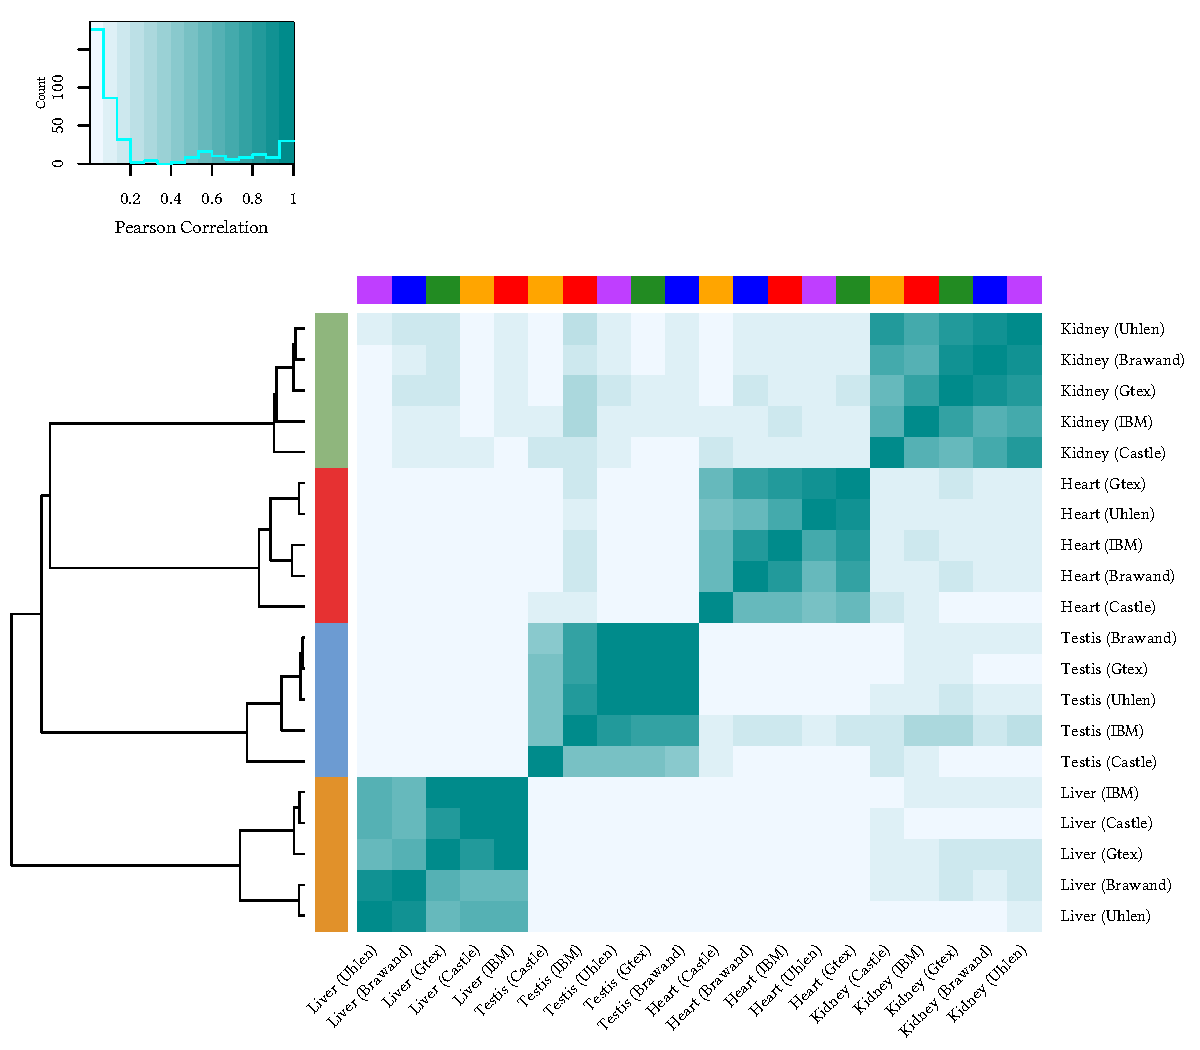
\includegraphics[scale=0.84]{transcriptomics/heatmap4TnoMitonoRep_1TC.pdf}\centering
    \caption[Heatmap of the 4 common tissues across the 5 studies]%
    {\label{fig:noMitoNoRep4T}\textbf{Heatmap of the four common tissues
    across the five studies.}\\All \pcgs\ (except the mitochondrial
    ones) at least expressed at 1 \FPKM\ are included.\\All the
    different \treps\ cluster by tissue of origin (y-axis colourbar)
    (instead for example by studies that is represented on the x-axis colourbar).}
\end{figure}

\begin{figure}[!htpb]
    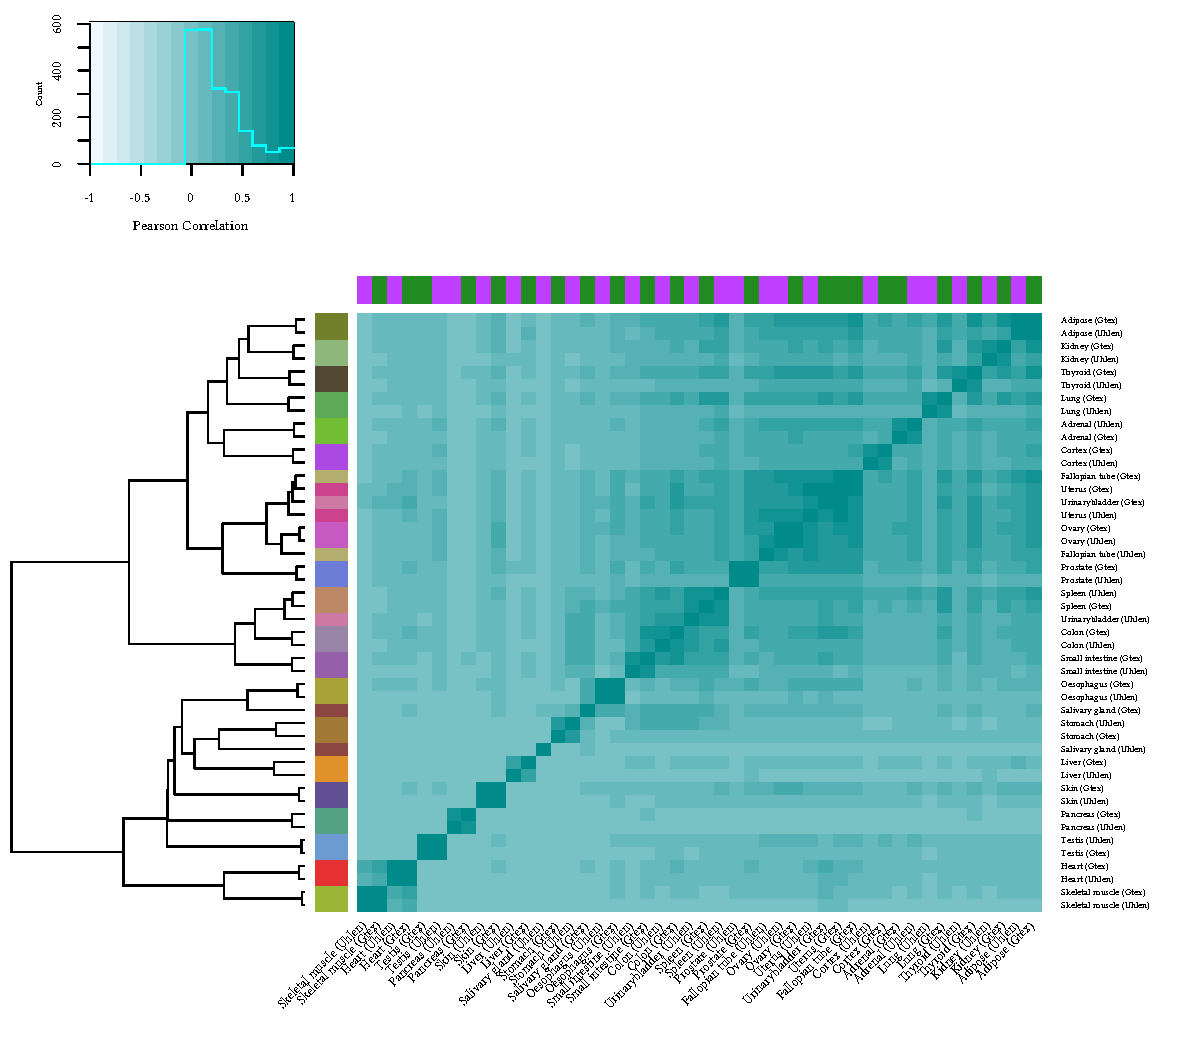
\includegraphics[scale=0.84]{transcriptomics/heatmap23TnoMitonoRep_1TC.pdf}\centering
    \caption[Heatmap of 23 common tissues between Uhlén and GTEx studies]%
    {\label{fig:noMitoNoRep23T}%
    \textbf{Heatmap of twenty-three common tissues between Uhlén and GTEx studies.}
    All \pcgs\ (≥ 1 \FPKM\ with the exclusion of the mitochondrial
    genes) are included.\\Most \treps\ cluster by tissues (y-axis colourbar)
    except for a few exceptions:
    There is a mixture of the \fallopian\
    and \Ovary\ \treps.
    In addition, \Salivary\ \treps\ is more correlated to
    \Esophagus\ or \Stomach\ regarding the original study.
    \Bladder\ \treps\ seem to cluster randomly with the others.
    However, these \treps\ are in singleton groups.}
\end{figure}

\Cref{fig:SamedistribPearsCorr} shows the distribution of the Pearson correlation
coefficients for the pairs of identical tissue profiles (\treps)
sourced from the different studies
for both of the working datasets \setOne\ and \setTwo.
Even with the lack of any batch effect correction,
most of the Pearson correlations are above 0.5.
Indeed,
there are two exceptions: the
correlation between the \Testis\ \treps\ of \castle\ and \vt\ (0.42)
for the 4-tissues working set and
\Salivary\ \treps\ of \uhlen\ and \gtex\ (0.2)
for the 23-tissues working set.
The median correlation for the four common tissues across the five datasets is
about 0.7 and 0.84 for the twenty-three tissues between \uhlen\ and \gtex\ studies.
Results are even better with Spearman Correlation:
the averages are respectively 0.49 for the 4-tissues sets
and 0.9 for the 23-tissues set and
the median correlations are 0.88 and 0.93.
As I mentioned in \Cref{ch:expression},
Pearson correlations are easier to understand and interpret
while Spearman correlations are more robust and thus better fitted for interstudy
comparisons.
See \Crefu{subsec:PearsonVsSpearman}.

\label{seg:betterTreps}
Both the Pearson\footnote{Despite one major outlier in the second
working set (\tissue{Salivary gland} --- Pearson correlation: 0.2)} and the
Spearman correlation coefficients for the more exhaustive 23-tissues working set
\setTwo,
comprising the two most recent studies,
are higher than the observed correlation for the 4-tissues working set.
Three main reasons may explain this situation:
\begin{itemize}[topsep=0pt,nosep]
    \item In addition to using paired-end sequencing,
        the library preparation protocols were better established
        for these two more recent studies;
    \item The instrument used for the sequencing were
        from the same series (HiSeq~2000 and HiSeq~2500); and
    \item These studies present a higher number of replicates per tissue.
\end{itemize}

\begin{figure}[!htpb]
    \includegraphics[scale=0.55]%
{transcriptomics/TransPearsonDistributionIdenticalOnly.pdf}\centering
\caption[Distribution of the correlations of same tissue pairs for the 4 and 23
tissues working sets.]{\label{fig:SamedistribPearsCorr}\textbf{Distribution
of the Pearson correlation coefficients of same tissues pairs for the four and
the twenty-three tissues working sets.}
In general, the Pearson correlations are high when we are
\emph{directly} comparing \treps\ from different studies.\\
The same-tissue pairs in the 23-tissues working set (\setTwo) present
a higher median correlation ($0.85$)
and narrower distribution than
in the 4-tissues working set (\setOne) (median$ = 0.74$).
However, \setTwo\ displays one outlier with
a very low Pearson correlation ($0.2$: \salivary\ tissue).
Sampling, processing differences or biological reasons
may just as well explain this outlier.}
\end{figure}

On the other hand,
the pairs comprising different tissues are very lowly correlated in general
(see \Cref{fig:distribCorr}).
Although, in a few cases of \setTwo\ (23-tissues working set),
high correlations are also observed for different-tissues pairs,
\eg\ \Fallopian\ and \Uterus\ from \gtex\ study
(see also \Cref{fig:noMitoNoRep23T}).
It is rather hard to decipher if this may be due to a technical issue
(\eg\ at the collection or library preparation stage)
or because these tissues are biologically very close.

\section{Possible driving force of the closer intratissue rather than intrastudy
similarity}

Since \Rnaseq\ allows distinguishing the shared biological origin
of most \treps\ across different studies,
the question then arises as to what is driving these strong interstudy
correlations.

As discussed in \Cref{sec:ExpressedOrNot}: \nameref{sec:ExpressedOrNot},
Pearson correlation coefficients measure the dependence between two tissue profiles (\treps)
and are subject to outliers and the skewness of the distributions.
As I have excluded the \emph{undefined}\footnote{I.e.\
\emph{unobserved} --- See also
\Cref{subsec:ExpressedOrNot-undefined}: \nameref{subsec:ExpressedOrNot-undefined}}
genes from the analyses,
the high correlations have another rationale than spurious null values.
Thus, the next intuitive step is to test
whether a particular subset of the genes may drive the correlation coefficients,
\ie\ are the highest, the most variable or another group of genes
the underlying reasons of the strong correlations.

\subsection{Highest expressed genes}

The notion of highest expressed genes may seem trivial,
but it depends on the normalisation method.
\Cref{ch:background} presents how all \Rnaseq\ values are inherently relative
to the observed genes and the normalisation assumptions.
Thus, from a same unnormalised (\ie\ \emph{raw count}) sample,
depending on the chosen normalisation
(see \Cref{subsub:norm}:~\nameref{subsub:norm}),
gene expression values and their final ranked order may be very different.
To minimise, if not avoid, such biases,
I have processed the data with consistent methods and annotation
and excluded selected sets of
genes\footnote{See \Cref{sec:bias_sources}:~\nameref{sec:bias_sources}}.
%Incidentally, if I pick another normalisation than \FPKM\footnote{See
%\Cref{eq:rpkm-fx}},
%the exclusion filters may impact a different set of genes.

To test how the highest expressed genes may influence the correlation,
I chose to visualise how the correlation trends vary
when I increase the expression threshold for the genes included
in the correlation calculation.
Thus, for \Cref{fig:CorHighExp4T} and \Cref{fig:CorHighExp23T},
I computed correlations of genes that are expressed above a cut-off
for each possible corresponding tissue pair of both working datasets \setOne\ and \setTwo.
The cut-off is a range (with step 10) of possible values (integers) of gene expression.

\begin{sidewaysfigure}[!htpb]
%\begin{figure}[!htpb]
    \centering
    \begin{subfigure}[b]{0.48\textwidth}\centering
        \includegraphics[width=\textwidth]{transcriptomics/HeartEvolHighExp4P-1}
        \caption{Heart}\label{fig:CorHighExpHeart4T}
    \end{subfigure}%
~%
    \begin{subfigure}[b]{0.48\textwidth}\centering
        \includegraphics[width=\textwidth]{transcriptomics/KidneyEvolHighExp4P-1}
        \caption{Kidney}\label{fig:CorHighExpKidney4T}
    \end{subfigure}

    \begin{subfigure}[b]{0.48\textwidth}\centering
        \includegraphics[width=\textwidth]{transcriptomics/LiverEvolHighExp4P-1}
        \caption{Liver}\label{fig:CorHighExpLiver4T}
    \end{subfigure}%
~%
    \begin{subfigure}[b]{0.48\textwidth}\centering
        \includegraphics[width=\textwidth]{transcriptomics/TestisEvolHighExp4P-1}
        \caption{Testis}\label{fig:CorHighExpTestis4T}
    \end{subfigure}
    \begin{subfigure}[b]{\textwidth}\centering
        \includegraphics[width=\textwidth]{transcriptomics/LegendEvolHighExp4P}
    \end{subfigure}
    \caption[Pearson correlation coefficient trends based on the expression
    levels of the genes considered for \setOne]{%
\label{fig:CorHighExp4T}\textbf{Pearson correlation coefficient trends
    based on the expression levels of the genes considered for each of the tissues
    of \setOne.}}
%\end{figure}
\end{sidewaysfigure}

For the 4-tissues working set \setOne\ (\Cref{fig:CorHighExp4T}),
except for very few pairs, the highest correlations correspond to
the lowest cut-off of 1 \FPKM\@.
In fact, the same tissue \trep\ correlation coefficients
are decreasing as the expression cut-off is increased
(the calculations involve then fewer genes).
Here below, the few exceptions grouped by tissue:
\begin{eqlist}[\eqliststarinit\def\makelabel#1{\bfseries#1}\labelsep1em]
\item[Heart] \uhlen{}-\gtex\ pair
\item[Kidney] \uhlen{}-\gtex, \castle{}-\uhlen\ and \castle{}-\gtex\ pairs,
\item[Liver]  \vt{}-\ibm, \ibm{}-\uhlen\ and \ibm{}-\uhlen\ pairs;
\item[Testis] \ibm{}-\uhlen, \vt{}-\gtex, \vt{}-\uhlen\ and \uhlen{}-\gtex\ pairs
\end{eqlist}

In the context of the 23-tissues working set (\setTwo) (\Cref{fig:CorHighExp23T}),
many more tissue pairs present very high correlation for subsets of their highly
expressed genes, \ie\ \skeletal, \Thyroid, \Cortex, \Uterus, \Kidney.
Unfortunately, these specific examples are insufficient
to derive any consensual threshold for future work.
Moreover,
for any similar tissue pair of \setTwo,
considering every \pcg\ expressed at least at 1 \FPKM\ is usually
far better than selecting any highly expressed genes subset
(except for \kidney).

\begin{figure}[!htpb]
    \includegraphics[scale=0.8]{transcriptomics/T23EvolHighExp23P.pdf}\centering
    \caption[Pearson correlation coefficient trend based on the expression
    levels of the genes considered for each of the 23 common tissues]{%
\label{fig:CorHighExp23T}\textbf{Pearson correlation coefficient trend based
on the expression levels of the genes considered
for each of the twenty-three common tissues between \uhlen\ and \gtex.}
In almost every case the complete set of common expressed \pcgs\ of each tissue gives
the highest correlations.}
\end{figure}

\setTwo{}'s results should be interpreted more carefully as
there are only two studies involved and
there are no actual means to distinguish
between an artefact or a true biological reason
that may drive the higher correlations.

Both for \Cref{fig:CorHighExp4T,fig:CorHighExp23T},
it seems that a couple of \treps\ are perfectly anticorrelated
for subsets of highest expressed genes,
These are most likely mathematical artefacts.
The correlation calculations are involve very few genes
and as such the correlations are more sensitive to any change
(see \Cref{sec:whyAnticor}).

As the interstudy Spearman correlations of same tissue pairs
are higher than the Pearson ones (\Cref{fig:distribCorr}),
I have explored the ratio of the common most top expressed
genes across the studies to the number of genes considered
(see \Cref{sec:overlapHighExp}).
The general trend of the overlap ratio for \setOne\ follows a random one
(\Cref{fig:highExpress4T}).
Indeed, only the top highest \pcgs\ in each tissue (about 10--20)
present high overlap ratios between the studies.
All the other \pcg\ ranks are indistinguishable from any random ordering.
\setTwo\ improved overlap ratio trend may solely be
the result of the smaller number of considered datasets
(see \cref{fig:highExpress4T}).

Together, these results indicate
that the highest expressed genes are unable to explain
the intratissue/interstudy high correlations.
Thus, I have considered other candidates
such as the most variable genes.


\subsection{Most variable genes across tissues}
As correlations translate the relationship strength,
similar gene expression variation patterns for the tissues
across the independent studies can also explain the strong correlations.
Moreover, other things being equal,
Pearson correlations are higher
when the range of observations has a broader variability scale.
This effect is often referred as
the \emph{restricted range}.~\mycite{CorrelationImpactingFactors}

There are several available estimators to describe the gene expression variability,
\eg\ the standard deviation~(sd) the variance~($sd^2$) or the coefficient of
variation~($\frac{sd}{mean}$).
I only report here the results based on the coefficients of variation.
The \gls{cv} allows assessing
the dispersion of the gene expression values
across the tissues within each dataset.
As it adjusts for the mean,
it is a more straightforward estimator to interpret than
the (standard) variance itself,
in particular for interstudy comparisons.

\begin{comment}
Visualising the \gls{cv} distribution of
gene expression for the working set \setOne\ (see \Cref{fig:HistCV4T})
allows determining whether they are similar across the five transcriptomic studies
or that inferring conclusions requires more cautions.
\end{comment}
As depicted in \Cref{fig:HistCV4T} (and \Cref{fig:HistCV23T}),
the distribution of gene expression \cvs\ presents a similar pattern
across the five studies of \setOne.

\begin{figure}[!htpb]
    \captionsetup{singlelinecheck=off}
    \includegraphics[scale=0.75]{transcriptomics/distributionCV_4commonTissues.pdf}%
    \centering
    \caption[Coefficients of variation across the 5 studies for the set of common
expressed genes and tissues]{\label{fig:HistCV4T}\textbf{Distribution of the
\cvs\ (cv) across \setOne\ (common set of expressed \pcgs\
across the four common tissues):
\{\Heart, \Kidney, \Liver, \Testis\}
across the five studies.}\\
The coefficients of variation (\gls{cv}) of the \pcgs\ (12,268) of the four tissues
present the same bimodal distribution profile across the five studies.
\\These profiles present two peaks: at $0.5$ and $2$.\\
Genes with a \gls{cv} lesser than or equal to $0.5$ have
a similar expression profile to a left-truncated version of
the complete gene set ones (due to the $1$ \FPKM\ cut-off)
as in \Cref{fig:distribPlot}.
On the other hand, the \pcgs\ with a coefficient of variation
equal to or greater than $1.5$ have two kinds of distinct profiles:
{\small
\begin{itemize}[topsep=0pt,nosep,leftmargin=95pt,listparindent=5pt]
    \item The gene expression is low across the four tissues, and
        it is above the cut-off of $1$ \FPKM\ only once
        (see \Cref{fig:mostVarBreadth}); or
    \item The gene expression is specifically high for one single tissue
        relative to the three others (See \Cref{fig:highestCVhist}).
\end{itemize}
}}
\end{figure}

\begin{figure}[!htbp]
    \includegraphics[scale=0.75]{transcriptomics/distributionCV_23commonTissues.pdf}\centering
    \caption[Coefficients of variation across \setTwo\ 2 studies and their set
    of common genes across the 23 tissues]{\label{fig:HistCV23T}\textbf{Distribution
    of the \cvs\ across \setTwo.}
    The bimodal distribution is more unbalanced than in \Cref{fig:HistCV4T}.
    Indeed, as more tissues are included for the calculation of the \cvs,
    the second peak is found around $5$.
    This peak has a smaller amplitude than the peaks at $2$ in \Cref{fig:HistCV23T}.
    There are still many genes that have a \cv\ around $2$.
    However, the overall distribution of the higher \cvs\ is smoother than
    for \setOne.
    Hence, most genes present a similar profile of expression through the various
    tissues.}
\end{figure}

The five datasets present two peaks.
One at approximatively 0.5 which characterises genes
that are quite invariant in their expression across the four tissues within each
dataset.
Another subset of genes forms peak for the \cvs\ equal to 2.
This last group of genes are the most variable ones in each dataset.
While there is some overlap of the most variable genes
between the five datasets,
it is only partial (see further \Cref{fig:cvEvol5DF}).


While \Cref{fig:noMitoNoRep23T} has already established that
the tissue expression profiles are very similar,
\Cref{fig:HistCV23T} highlights that most genes seem to share the same
intertissue expression profile variability as the distribution of the coefficients
of variation across \uhlen\ \etal\ and \gtex\ studies are very alike.

A simple approach to test if the common most variable genes
are the driving force of the correlation is
to study the difference of their correlation with
the remaining set of considered \pcgs.
If the most variable \pcgs\ are driving the correlation,
then their group has to present higher correlations than the second set.

After ranking the \pcgs\ in decreasing order of their \cv\ within each study,
I select the intersection of genes in the first quarter across them
to create the set of most variable genes $S_{most~Variable}$.
The remaining genes are constituting the second group $S_{remaining}$\footnote{%
$S_{remaining} = $ \setOne{}$- S_{most~Variable}$}.
For both of these gene groups, $S_{most~Variable}$ and $S_{remaining}$,
I calculate the coefficients of correlation for all possible tissue couples.

\begin{figure}[!htpb]
    \includegraphics[scale=0.7]%
    {transcriptomics/TransPearsonDistributionIdenticalDifferentHighestCVgenes.pdf}%
    \centering
    \vspace{-0.2in}
    \caption[Comparison between the most variable genes with all the other ones]%
    {\label{fig:test_mostvaribleVSevery}\textbf{Comparison between
    the most variable \pcgs\ with the remaining genes in \setOne\ set.}
    For both the most variable group $S_{most~Variable}$
    and the remaining one ($S_{remaining}$) of \pcgs,
    the correlations between identical interstudy tissues are significantly greater
    than any correlation between different (even intrastudy) tissues
    (see respective p-values).
    The distribution of the intertissue correlations for $S_{most~Variable}$
    shows that these genes are showing a tissue signature
    while they lack an interstudy linear relationship for same tissue
    couples.% {\footnotesize The correlations between different tissues pairs
    %are provided for control purposes.}
    }
\end{figure}

\Cref{fig:test_mostvaribleVSevery} summarises this analysis.
It shows the Pearson correlation distribution
for these two groups of \pcgs\ in \setOne.
One-sided \Welchttest\footnote{See \Cref{mini:ttest}.}
allows rejecting the null hypothesis $H_0$ at 95\% of confidence.

The mean of the %(Pearson and Spearman)
correlation coefficients
calculated with the common most variable \pcgs\ is significantly greater than
the ones calculated with the remaining set of \setOne\ genes ($H_1$)%\footnote{Though,
%a two-sided \Welchttest\ compels one to accept the $H_0$ hypothesis:\\
%the two populations of coefficients correlation are not significantly different
%(\pvalue{= 0.07}).}%
.

For Pearson correlation:
$mean_{S_{most~Variable}}=0.76$ and $mean_{S_{remaining}}=0.68$
(\pvalue{= 0.03}).
Thus, the common \pcgs\ with the highest \cv\
discriminate better between the identical and different tissues.

Though, for both groups,
$S_{most~Variable}$ and $S_{remaining}$,
the \treps\ across the studies cluster mostly by tissue rather than
original study.
See and compare \Cref{fig:heatmapMost25pVariable,fig:ReverseheatmapMost25pVariable}.
These supplementary figures respectively present
the heatmaps (with clusterings) of the tissues
based on their Spearman correlation for the most variable (\cv) \pcgs\
and all other remaining genes of \setOne.
The \treps\ cluster mainly by their original tissue.
In fact, the only exception is that
\castle\ tissues cluster primarily by study
once I exclude the most variable genes.

To avoid any oversight due to the arbitrarily chosen number (first quarter)
of the most variable genes,
I have also studied the course of the intersection size of the common genes
across the five studies
as a function of the number of \setOne\ genes that I consider.
\Cref{fig:overlapConcept} illustrates my general approach.
After ordering the genes by decreasing order of their \cv\
within each of the datasets comprised in \setOne,
I have calculated the size of overlap for each rank (\ie\ from 1 to 12,268)
between the five datasets.
To help with the interpretation,
I finally divide the previous figure by the rank.

\begin{figure}[!htpb]
    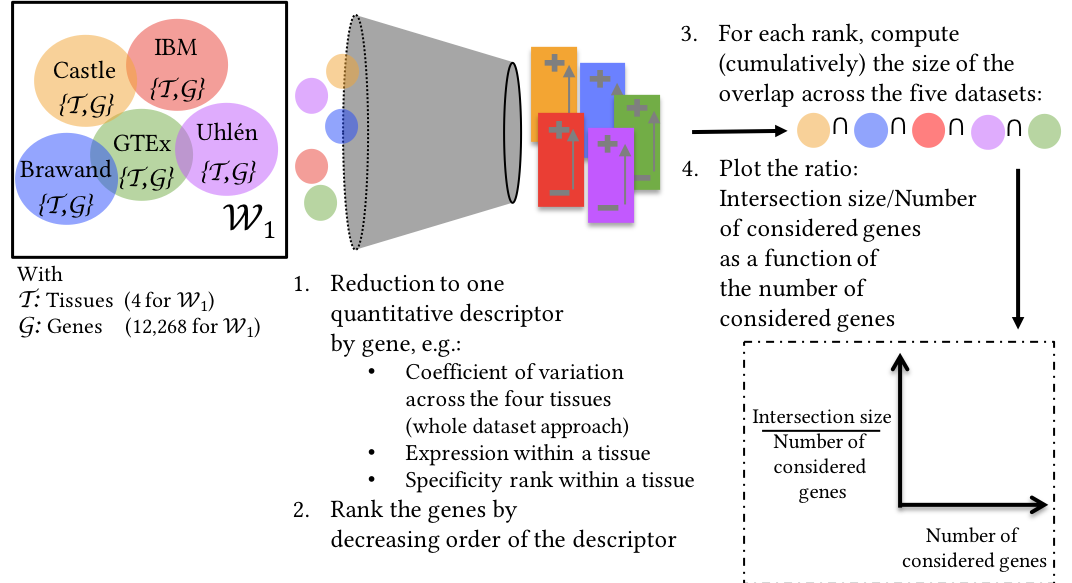
\includegraphics[scale=0.9]{transcriptomics/ConceptOverlap.png}\centering
    \caption[Overview for the comparison of the genes across the five
    studies based on a ranked descriptor 5 studies]{\label{fig:overlapConcept}%
    \textbf{Overview for the comparison of the genes across the five
    studies based on a ranked descriptor.}
    The first step applies individually to each of the studies
    within the working dataset (\ie\ here \setOne).
    It consists in extracting a single value per gene
    (\eg\ a statistic or any other quantitative descriptor)
    either for the entire \emph{d}ataset (referred thereafter as \emph{D-approach}) or
    for each \emph{t}issue in each dataset (referred as \emph{T-approach}).
    The next steps include
    computing (cumulatively) the intersection size number for each rank
    and plotting this number divided by the rank
    in function of the number of considered genes (\ie\ rank).}
\end{figure}

\Cref{fig:cvEvol5DF} presents the result.
Many of the most variable genes are commonly present in the top tier of the
five studies, though they have different individual rank.
Indeed, there is a strong growth for about the first 1,250 genes that then
settles a plateau which increases toward the final ratio ($1$).
Using the first quarter of the most variable genes as a cut-off appears
to be an acceptable threshold
as it comprises the initial growth and part of the plateau.

\begin{figure}[!ht]
    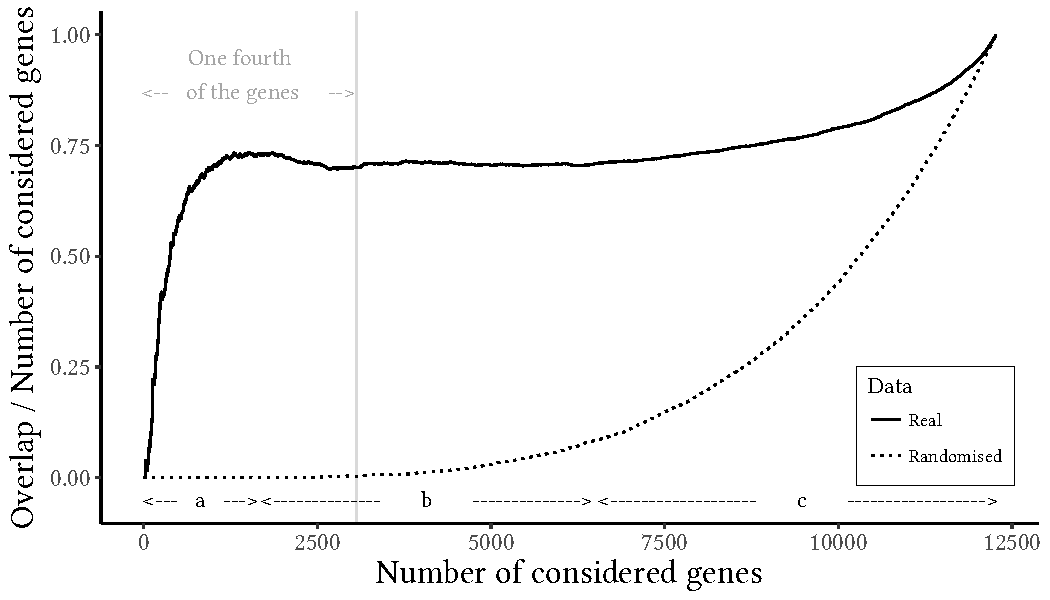
\includegraphics[scale=0.9]{transcriptomics/CVevolCumul5DF_line-abc.pdf}\centering
    \vspace{-0.15in}
    \caption[Intersection size of \setOne\ genes (ranked by cv)]%
    {\label{fig:cvEvol5DF}\textbf{Intersection size course
    of \setOne\ genes (based on their coefficient of variation rank
    in each of the five studies).}
    There are three main parts.
    There is an initial strong growth (a)
    %followed by a short plateau (b)
    %before a slight decrease (c)
    which then settles a plateau (b).
    Eventually, the ratio increases slowly again
    until reaching the expected ratio of $1$ once all the genes from \setOne\
    are included (c).
    The first quarter of the genes covers (a) and a part of (b).
    Apart from (a),
    the overlap of shared genes between the five datasets when ranked on their
    coefficient of variation is above 70\%.
    The sigmoid curve (dashed line) is based on randomised data
    where permutations break the original order of the genes. (Within each dataset,
    all the gene expression levels are permuted within each tissue,
    \ie\ the overall pattern of expression of each tissue is conserved.
    This operation is performed 10,000 times.
    The dashed line is a summary of all these permutations).
    There is a distinct dissimilarity between the real and the randomised data.}
\end{figure}

\begin{figure}[!ht]
    \captionsetup{singlelinecheck=off}
    \includegraphics[scale=0.9]{transcriptomics/CVevolCumul2DF_line-abc.pdf}\centering
    \caption[Intersection size of \setTwo\ genes (ranked by cv)]%
    {\label{fig:cvEvol2DF}\textbf{Intersection size course
    of \setTwo\ genes (based on their coefficient of variation rank
    in each of the two studies).}
    Globally, there are two parts: one initial strong growth (a) and
    a second part (b) where the curve shifts shallowly towards
    the expected final ratio of 1.
    While the number of genes involved in \setTwo\ is higher than in \setOne,
    the ratio of common genes that are the twentieth most variable in each study
    is above 75\%.
    There are three main reasons that may explain this improved result compared
    to \Cref{fig:cvEvol5DF}.%
    {\small%
    \begin{itemize}[topsep=0pt,nosep,leftmargin=95pt,listparindent=5pt]
       \item \setTwo\ involves a smaller degree (\ie\ number of studies)
           than \setOne\ (respectively 2 and 5).
           Hence, bigger intersection sizes are easier to occur.
       \item As previously mentioned, \gtex\ and \uhlen\ studies provide probably
           more accurate \treps\ than the other studies (see~\vref{seg:betterTreps}).
       \item The greater number of tissues induces a wider range of \cvs,
           which allows picking up genes with more subtle variations.
   \end{itemize}}
    }
\end{figure}

\begin{comment}
If the previous analysis was to include
only the first 1,250 most variable genes
the results of \Cref{fig:heatmapMost25pVariable} may be even greater.
However, the dissimilarities highlighted by \Cref{fig:ReverseheatmapMost25pVariable}
would also be greater.
\end{comment}

In conclusion, while the most variable genes have a significant influence
on the strong and biologically meaningful correlations,
there must be other gene categories contributing.

One main drawback when considering the most variable genes is
that the coefficient of variation (as any other statistics)
may significantly vary
depending on the composition of the working set.
Thus, this analysis may need to be rerun.

\subsection{Genes with tissue-specific (TS) expression}\label{sub:TisSpeGene}
\vspace{-.25in}
Another good candidate to drive higher correlations
between identical tissue interstudy \treps\ than intrastudy different ones
are the genes that have an expression profile
that varies according to the tissues.
As reported before,
most \mRNAs\ are expressed in every tissue~\mycite{ramskoldan:2009}
(see also \citet{Uhlen2015,GTExTranscript} for other examples) and
their expression is relatively invariant across the tissues (\Cref{fig:HistCV4T}).
Moreover,
many of the most variable genes
have a regular gene expression across the different tissues
from aside one or two where the expression is notably higher globally
(see \Cref{fig:expressionMostvariableG}).
Thus,
considering genes with a \gls{TS} expression
seems a reasonable approach to explain the high correlations.

The definition of tissue specificity is unclear and
varies from one study to another (see also \citet{Santos2015-rj}).
\citet{Liang2006-mk} define \emph{tissue specificity}
only for genes expressed solely in one tissue,
and then \emph{tissue selectivity} for genes expressed in more than one tissue
with an expression enriched in one or a subset of tissues.
Other studies have a broader definition of tissue specificity.
They identify genes above a given threshold of tissue selectivity (or enrichment)
as tissue-specific genes.
See for examples \citet{Uhlen2014,Jiang2016-sv}.
In this second case,
genes with a single-tissue expression are an extreme case of \gls{TS} genes.

Within this thesis, I use the second definition,
\ie\ I consider genes as \gls{TS}
as long as they display a higher tissue selectivity than a preset threshold,
regardless of how many tissues express them.
Indeed, every study presents a subset of genes
that are expressed above 1 \FPKM\
in a sole tissue (see \Cref{fig:breadthGenesP1}).
However, the decreasing number of these genes
when increasing the number of considered tissues highlights
the arbitrary relativity introduced by the study design.

Even for the second definition only,
there are many methods to characterise genes tissue-specificity.
See \citet{Cavalli2011-bo,Xiao2010-mz,Karthik2016-mu,Kim2017-dz,%
Kryuchkova-Mostacci2017-mk,Kadota2006-eb,Yu2006-ha,Martinez2008-bm}
for some examples.
There are also databases that record previously identified \gls{TS} genes,
for normal conditions,
\eg\ \WebFoCi{TiGER}{http://bioinfo.wilmer.jhu.edu/tiger/}{tiger} or
\WebFoCi{TiSGeD}{http://bioinf.xmu.edu.cn:8080/databases/TiSGeD/index.html}{Xiao2010-mz}
and more specialised ones, \eg\ for cancer
\WebFoCi{TissGDB}{https://bioinfo.uth.edu/TissGDB/index.html}{Kim2017-dz}.

Amongst all the possible approaches to characterise the \gls{TS} \pcgs,
I detail three that I used in the following subsections.
First, I have queried \gls{TIGER} to capitalise on previous knowledge.
Then, to derive the \gls{TS} genes directly from \setOne\ and \setTwo,
I have used a published method,
that uses the gene expression \emph{fold change} (FC) ratio across the tissues.
Finally, I have employed a robust method designed to detect outliers in data,
\ie\ Hampel's test \mycite{Hampel1974},
to identify genes which present an unusual expression level in a single tissue.
In fact, as gene tissue selectivity and tissue specificity definitions are
relative to a context,
if the latter changes,
the genes attributes may change as well
(\eg\ one gene that is unspecific in \setTwo\ may be \heart{}-specific in \setOne).


\subsubsection{Use of prior knowledge: TiGER database}\label{subsub:Tiger}

\gls{TIGER}~\mycite{tiger} reports \gls{TS} genes for thirty independent tissues
(based on \glspl{EST} experiments).

After retrieving the list of genes for all reported tissues,
I have mapped the \gls{Refseq} identifiers provided by \gls{TIGER}
to \gls{Ensembl} gene identifiers (\hg{38}, \ens{76}).
Then, I removed all duplicates due to the identifier translation within each tissue,
and I also filtered out all the genes identifiers that
I found in more than one tissue:
\gls{TIGER} lists a subset of the same genes in many tissues,
but the modification in the annotation may also explain part of the
repetitive genes.
Thus, for each tissue,
I have a list of identifiers that are specific to that tissue only.

\begin{figure}[!ht]
    \includegraphics[scale=0.9]{transcriptomics/Tiger5DF4Tissues.pdf}\centering
    \vspace{-.15in}
    \caption[Expression heatmap of the four tissues across the five datasets based on
    TiGER]{\label{fig:TigerGenes}\textbf{Expression heatmap of the four tissues
    across the five datasets based on \gls{TIGER} information.}
    This heatmap illustrates three subsets of genes:
    genes for which real expression data confirm their \gls{TIGER} definition;
    genes failing to show any \gls{TS} profile in their expression data; and
    genes with mismatching tissue specificity between \gls{TIGER}
    definition and the expression data.
    The colourbar above the heatmap is representing the tissue
    for which \gls{TIGER} annotates the genes (presented as columns) as \gls{TS}
    (red for \Heart, green for \kidney, light orange for \liver\ and blue for \testis).
    \gls{TIGER} definitions are of variable accuracy.
    }
\end{figure}

\Cref{fig:TigerGenes} is an expression heatmap based on
a subset (\ie\ $916$)  of \pcgs\
that are present in this final list of translated \gls{TIGER} genes
for the  \heart, \kidney, \liver\ and \testis.
There are three main types of genes.
The largest group comprises the genes with a corroborating profile
between the \gls{TIGER} definition and the real data.
Then, a second smaller group encompasses genes
listed as \gls{TS} in \gls{TIGER},
but fail to demonstrate expression specificity
towards any tissue in the real data.
Finally, the third group includes a very tiny subset of genes which
are more specific to another tissue than the initially stated one.

Thus, without any additional knowledge,
it is difficult to predict beforehand which original \gls{TIGER} definitions
will be confirmed or denied by expression data.
Remarkably, most of the genes present the same expression pattern
through the tissues across each of the studies
and thus regardless of their \gls{TIGER} category.
Once again, \castle\ expression data is exhibiting
the only few observed discrepancies\footnote{Reminder:
the \gls{FPKM} quantification (used here) is sensitive
to the number of identified genes (see \Cref{eq:rpkm-fx}~\vref{eq:rpkm-fx})
and \castle\ study identifies and quantifies many more \glspl{RNA} than the
other studies as it uses a whole \RNA\ protocol
while the others are using polyA-enrichment (see \Cref{ch:datasets}).}.

\subsubsection{Fold change method}\label{subsub:TisSpeGeneMethodPerso}
As \citet{DESeq2} noted the most common approach for detecting
a gene expression difference between two conditions is
to study the expression fold change (FC) ratio between these conditions.
This approach is inappropriate for direct use
with differential study\footnote{I.e.\ treated (diseased)
versus control samples comparison study.}
designs and
needs corrections~\mycite{Anders2010-vq,DESeq2,Soneson2013-pd,edgeR}.
However, this method is still broadly present in the literature,
especially for studies other than differential gene expression analyses.
As examples, see~\citet{Uhlen2015,Zhu2016-xo,Yu2015-uh}.
Besides, \egxa\ \mycite{EBIgxa} relies on this method to select
the most specific genes for \emph{baseline} studies\footnote{In
contrast to differential gene studies,
the baseline studies focus on
depicting the expression landscape of each covered condition
instead of focusing on the gene expression through these conditions.}.
There are also a few variations
on how to compute this ratio (see~\citet{Zhu2016-xo,Uhlen2015}).

In this thesis,
I compute the FC ratio by dividing the expression
of each gene in a given tissue
by the maximum expression of this gene across all the other tissues of that study
in the working set.
Studies usually pick arbitrary cut-offs to characterise the specific genes.
\citet{Uhlen2015} uses cut-offs of $2$ and $5$ \FPKM\
to determine \emph{enriched} and \emph{enhanced} tissue genes.
\citet{Zhu2016-xo} set their cut-off at $2$ to characterise \gls{TS} protein-coding
and noncoding transcripts.
However,
I avoid arbitrary cut-offs, and
I use the FC ratio to rank the \pcgs\ of my working datasets according
to their specificity within each tissue:
higher FC ratios indicate genes with higher specificity.
I then assess the consistency of the tissue specificity of the genes through the
various studies.
For that, I have followed the \emph{T-approach} overviewed in \Cref{fig:overlapConcept}.

\begin{figure}[!pthb]
    \includegraphics[scale=1]{transcriptomics/mostSpe4TP1.pdf}\centering
    \vspace{-0.2in}
    \caption[Intersection size curve of \setOne\ genes based on their FC ratio
    rank in each tissue across the five studies]{\label{fig:mostSpe4T}\textbf{Intersection
    size curve of \setOne\ genes based on their specificity (FC ratio rank)
    in each tissue across the five studies.}
    When ranked by specificity in \heart, \kidney\ and \liver,
    one fortieth of \setOne\ \pcgs\ are commonly shared between the five studies.
    For \testis, the shared amount of genes reaches more than one-tenth of \setOne\
    whole set of genes.
    Compared to the most variable genes (\Cref{fig:cvEvol5DF}),
    the most specific genes seem to be more consistent across the studies.
    }
\end{figure}
\begin{figure}[!pbht]
    \includegraphics[scale=0.9]{transcriptomics/mostSpe23TP1.pdf}\centering
    \vspace{-0.2in}
    \caption[Intersection size curve of \setTwo\ genes based on their FC ratio
    rank in each tissue across the two studies]{\label{fig:mostSpe23T}\textbf{Intersection
    size curve of \setTwo\ genes based on their specificity (FC ratio rank)
    in each of the twenty-three tissues across the two studies.}
    }
\end{figure}

\Cref{fig:mostSpe4T} presents the shifts in the intersection size curves of the
four tissues of \setOne.
The most specific genes in each tissue of \setOne\ are shared between the
five studies.
Indeed, the slopes are very sharp before reaching a peak and dropping as sharply
for the first fortieth genes in \heart, \kidney\ and \liver.
The intersection of the most specific genes is even greater for \testis\ as
it concerns more than a tenth of \setOne\ genes.
\Cref{fig:mostSpe23T} shows that this observation seems to hold true
when the number of tissues and genes is increased.

Thus, the \gls{TS} genes are also contributing to provide a stronger
biological signal over the technical noise.

\subsubsection{Hampel's test: detection of \emph{atypical} expression}\label{subsub:Hampel}

Hampel's test is a robust method
for detecting outliers~\mycite{Davies1993-nv,Pearson2002-im}
in data that are identically and independently distributed (i.i.d.)~\mycite{Liu2004-kf},
while easy to implement and use~\mycite{LinsingerHampel}.
Much interlaboratory or interstudy research in the literature
\eg~\citet{LinsingerHampel,Lewczuk2006-wq,Rocke1983-qa,Apfalter1999-ca}
use this test to detect outliers.
The method uses the median, the \gls{MAD}\footnote{MAD:~median absolute deviation}
and a cut-off to define the observations that stand apart.

For this thesis, I have derived this test to identify conditions (\ie\ tissues)
where the gene expression is \emph{atypical}.
I rely on the two facts that
most genes are expressed everywhere \mycite{ramskoldan:2009,Uhlen2015,GTExTranscript}
(see also \Cref{fig:breadthGenesP1}),
and they mostly present a limited variation in their expression
through the various tissues (see \Cref{fig:HistCV4T,fig:HistCV23T}).
Thus, when the expression of the gene is atypical
(\ie\ an outlier to the average profile of that gene expression across the many tissues),
it denotes a tissue specificity.
Besides,
this test allows detecting genes that are over- or under-expressed in specific tissues,
whereas the other methods are only detecting the overexpressed genes.

After implementing the method (see \Cref{algo:hampel}, p.~\pageref{algo:hampel})
with a (widespread) adimensional cut-off of $5.2$, % (which assumes a normal-like distribution),
I have applied it to the whole original datasets and \setTwo.
\setOne\ comprises too few tissues to allow detecting \emph{atypical} expression.
Overall, there are always more than 60\% of congruence between the genes tagged
as atypical in a specific tissue for the whole dataset
and the subset of twenty-three tissue.
The proportion of agreement between the partial and whole datasets increases,
even more, when I filter the results to keep only the genes that are recurrently
picked for both \uhlen\ and \gtex\ data.
Thus, though known as a robust method,
Hampel's test outcomes are still dependent on the set of considered tissues.

\begin{figure}[!htbp]
    \includegraphics[scale=1]{transcriptomics/hampel5DF4Tissues.pdf}\centering
    \caption[Expression of the genes picked with Hampel method]{\label{fig:hampelExp}%
    \textbf{Expression of the genes picked consistently with the Hampel method
    in each study solely in one tissue.}}
\end{figure}

\Cref{fig:hampelExp} regroups the genes that the Hampel test detects
as outliers for the five studies for their four shared tissues.
All corresponding-tissue \treps\ present similar patterns of expression
regardless of their original study,
although the \castle\ \treps\ have overall lower expression values than the others.
Other filters may improve the results:
\eg\ selecting genes with higher expression or
increasing the cut-off above $5.2$ in selected tissues.

\subsection{Uhlén categories}\label{sub:UhlenGeneCat}

Put together the results from the previous sections seem to describe that
the strong correlations are driven by different categories of genes.

Uhlén laboratory publications \mycite{Uhlen2014,Uhlen2015,Uhlen:2016}
use different categories of genes to describe the normal human transcriptome.
As their classification changes between these related papers,
I have redefined a classification based on them
(presented in \Cref{tab:UhlenCat})
before applying it to \setOne\ and \setTwo\ (\Cref{tab:UhlenCategoriesProtCoding}).

\begin{table}[!htpb]
\centering
\caption[Gene classification]{\textbf{Gene classification}\label{tab:UhlenCat}\\
\footnotesize{adaptation of \uhlen\ \etal\ classification~\mycite{Uhlen2014,Uhlen2015,Uhlen:2016}}}
\begin{tabular}{@{}ll@{}}
\toprule
Category        & Definition                                                                                           \\ \midrule
Not detected    & Never detected above 0 FPKM                                                                    \\
Not expressed   & Never detected above 1 FPKM                                                                    \\
Mixed high      & Expressed in a subset of tissues and always $\geq 10$ FPKM                                     \\
Mixed Low       & Expressed in a subset of tissues and always $< 10$ FPKM                                 \\
Ubiquitous High & Expressed in all the tissues and always $\geq$ 10 FPKM                                         \\
Ubiquitous Low  & Expressed in all the tissues and always $< 10$ FPKM                                     \\
Group enhanced  & Expressed in a subset of tissues with an expression $\geq 5*mean_{all~the~tissues}$             \\
Tissue enhanced & Expressed in a single tissue with an expression $\geq 5*mean_{all~the~tissues}$                 \\
Tissue enriched & Expressed in a single tissue with an expression $\geq 5*Max_{all~the~other~tissues}$ \\ \bottomrule
\end{tabular}
\end{table}

\Cref{tab:UhlenCategoriesProtCoding} shows that for many of these categories,
the number of shared \pcgs\ is high between the different studies of the
two working datasets \setOne\ and \setTwo.
It supports the previous results that \pcgs\ present in general a similar
gene expression profile for a same set of tissues across studies.


\pagestyle{plain}
\begin{landscape}
\begin{table}[]
\centering
\caption[Uhlén et al.\ gene categories]{\label{tab:UhlenCategoriesProtCoding}%
\textbf{Uhlén et al.\ gene categories}\\
\footnotesize{Apart from the undetected genes and the ones expressed below 1 \FPKM,
a gene may be referenced in several categories.}}

%\begin{tabular}{@{}lllllllllll@{}}
\begin{tabular}{@{}ccccccccccc@{}}
\toprule
\multicolumn{2}{c}{\multirow{2}{*}{\begin{tabular}[c]{@{}c@{}}\ens{76}
    \\($\sim$22,500 protein\\coding genes) \end{tabular}}} &
\multirow{2}{*}{\begin{tabular}[c]{@{}c@{}}\\Not\\detected\end{tabular}} &
\multirow{3}{*}{\begin{tabular}[c]{@{}c@{}}Not expressed\\ at 1 \gls{FPKM}\\
    cut-off\end{tabular}} &
\multicolumn{2}{c}{Mixed expression} &
\multicolumn{2}{c}{Ubiquitous expression} &
\multirow{2}{*}{\begin{tabular}[c]{@{}c@{}}\\Group \\Enhanced\end{tabular}} &
    \multirow{2}{*}{\begin{tabular}[c]{@{}c@{}}\\Tissue\\ Enhanced\end{tabular}} &
        \multirow{2}{*}{\begin{tabular}[c]{@{}c@{}}\\Tissue\\ Enriched\end{tabular}} \\
    \cmidrule(lr){5-8}
\multicolumn{2}{c}{}
    &  &  &
    \begin{tabular}[c]{@{}c@{}}Low\\ (\textless\ 10 \gls{FPKM})\end{tabular} &
        \begin{tabular}[c]{@{}c@{}}High\\ (≥ 10 \gls{FPKM})\end{tabular} &
            \begin{tabular}[c]{@{}c@{}}Low\\ (\textless\ 10 \gls{FPKM})\end{tabular} &
    \begin{tabular}[c]{@{}c@{}}High\\ (≥ 10 FPKM)\end{tabular} &  &  &  \\
        \midrule
        \multicolumn{1}{c}{%
        \multirow{6}{*}{\rotatebox[origin=c]{90}{\parbox[c]{3cm}{\centering Whole
        dataset}}}} &
        Castle & 3,403 & 3,268 & 8,773 & 1,033  &
        1,399  & 634   & 11   & 3,664   & 1,975 \\
        \multicolumn{1}{c}{} & Brawand & 2,964 & 3,095 &
        8,034 & 1,788  & 1,760 & 958   & 0  &
        2,729  & 2,548 \\
        \multicolumn{1}{c}{} & IBM & 2,693 & 2,605  &
        7,325  & 1,406  & 1,135 & 858  & 322 &
        5,248  & 2,453  \\
        \multicolumn{1}{c}{} & Uhlén & 2,662 & 1,747 &
        5,769 & 1,053  & 456 & 406  & 2,511  &
        5,201  & 2,333  \\
        \multicolumn{1}{c}{} & GTEx & 2,197  & 1,886  &
        5,556  & 1,117 & 687  & 698  & 3,859  &
        4,356  & 1,919 \\ \cmidrule(l){2-11}
        \multicolumn{1}{c}{} & Consensus & 2,197 & 486  &
        1,749  & 221  & 33  & 161  & 0  & 677  &
        \begin{tabular}[c]{@{}c@{}}531 %$[$518$]$
        \end{tabular} \\
            %\multicolumn{1}{c}{} & \footnotesize{without Gtex} &
            %\footnotesize{2,413} & \footnotesize{638} & \footnotesize{2,152} &
            %\footnotesize{286} & \footnotesize{63}  & \footnotesize{179} &
            %\footnotesize{0}  & \footnotesize{814} &  \footnotesize{587}  \\
            \midrule
\multirow{6}{*}{\rotatebox[origin=c]{90}{\parbox[c]{3.5cm}{\centering Common\\
4 tissues\\ Working datasets}}} &
Castle & 19,066 & 2,994 & 8,589 & 1,513 &
2,994 & 1094 & --- & --- & 2,185 \\
& Brawand & 19,505  & 2,962  & 8,626  & 2,228
& 2,962  & 1251 & --- & --- & 3,672  \\
& IBM & 19,776  & 2,989 & 8,534 & 1,954 &
2,989  & 1212  & --- & --- & 2,824  \\
& Uhlén & 19,807 & 2,917 & 8,367 & 2,227 &
2,917  & 1190  & --- & --- & 3,730  \\
& GTEx & 20,272 & 3,870 & 8,988  & 2,312 &
3,870  & 1427  & --- & --- & 3,554  \\
\cmidrule(l){2-11}
& Consensus & 1,973 & 550 & 3,351 & 649 &
550  & 439 & --- & --- & 1,412  \\
%& \footnotesize{without Gtex} & \footnotesize{2,413}  & \footnotesize{2,186}  &
%\footnotesize{3538}  & \footnotesize{639}  & \footnotesize{576}  &
%\footnotesize{439}  & \footnotesize{---} & \footnotesize{---} & \footnotesize{1,462}
\midrule
\multirow{3}{*}{\rotatebox[origin=c]{90}{\parbox[c]{1.7cm}{\centering Common\\ 23
tissues\\ Working datasets}}} & Uhlén & 2,662  & 1,970  &
6,160 & 1,135 & 594  & 427 & 1,285 &
5,776 & 2,518 \\
& GTEx & 2,197 & 2,258 & 6,966  & 1,540 &
1,822  & 997 & 1,048 & 5,496  & 2,460 \\
\cmidrule(l){2-11}
& Consensus & 2,197 & 1,544 & 4,936 & 791 &
423 & 417 & 558 & 4,223 & 1,885 \\
\bottomrule
\end{tabular}
\end{table}
\end{landscape}
\pagestyle{scrheadings}


\subsection{Curated sets}\label{subsec:Trans_curatedSets}
\Pcgs\ that were characterised consistently
as any of the aforementioned categories across the five datasets of \setOne\
or the two of \setTwo\
are provided digitally as supplementary data,
which can also be found at \url{https://www.barzine.net/~mitra/thesis}.
\\The code required to produce these results can be found at \github.


\section{Discussion}\label{sec:Trans_discussion}

In this chapter,
I have directly compared and integrated
the most extensive number to date of~\Rnaseq\ transcriptome
of normal human tissues based on samples from 5 studies together.
This allowed me to construct two working datasets of \pcgs.
The first one (\setOne) comprises four tissues
and 12,268 shared genes
extracted from five independent studies
(\cite{Krupp2012,VTpaper,Uhlen2015,GTExTranscript} and \ibm)
and the second one (\setTwo) comprises twenty-three tissues
and 17,554 shared genes
from two studies (\cite{Uhlen2015,GTExTranscript}).

Clustering analyses (and \Welchttest) of these two sets
confirm that \Rnaseq\ technical noise is
lower that relevant biological signals present in the data.
Indeed,~\cite{Sudmant2015-zt,Danielsson2015-cn,Yu2015-uh} and~\cite{Uhlen:2016}
also observe that interstudy corresponding tissues pairs are more related than
intrastudy non-corresponding tissue ones
(average correlation for corresponding tissue-pairs $r=0.75$, $\rho=0.88$;
average for non-corresponding tissue-pairs $r=0.20$, $\rho=0.75$).

In an attempt to inspect possible underlying forces for the close \treps\
similarities across the studies,
I have considered different attributes and groups of genes:
\emph{highest expressed}, \emph{most variable}, \emph{most specific}.
The top highest expressed genes show a very small (if any) impact on
the interstudy tissue expression profile strong correlations.
The most variable and most specific genes have a real contribution even though
their importance may be relative compared to the whole set of expressed genes.
As the definition of \gls{TS} genes is very variable from one study to another
(see \cref{sub:TisSpeGene}),
I have relied on three different methods to pick them,
including extracting \gls{TS} gene definitions
from an existent resource
\WebCi{TiGER}{http://bioinfo.wilmer.jhu.edu/tiger/}{tiger}
that I have updated to the current human genome build (\hg{38})
before using them within my thesis.
Mining the experimental data with this updated list highlights
the need for cautiousness when dealing with older resources.
While the congruence of the three methods is partial,
the \gls{TS} genes show distinct expression profiles across tissues
that are rather consistent through the different studies.

Finally, through a classification inspired
by Uhlén et al.\ \mycite{Uhlen2014,Uhlen2015,Uhlen:2016}
and which considers together the breadth, the level and the specificity of expression,
I have explored the congruence of the genes categories across the studies.

Concomitantly, other research groups have published similar studies
since I started this project.
However, at the time of writing this thesis,
all the other studies (including the aforementioned ones)
were still based on the human genome build \hg{37} (or hg19),
while I am using the more recent \hg{38} one.
These studies either have different focus, aims,
approaches or more limited scopes.
Thus, my work expands or completes theirs on different points as next explained.
\begin{itemize}[topsep=0pt,nosep]
%Feb 2016 -Uhlén
\item\fullcite{Uhlen:2016} In this review paper,
the authors present the results of \citet{Yu2015-uh} and \citet{Danielsson2015-cn}
discussed in following points.
They also compare the \gtex\ released data~\mycite{Bahcall2015-mh,GTEx_Consortium2015-si,Gibson2015-wh}
to their own~(\uhlen\ data~\mycite{Uhlen2014,Uhlen2015}).
As they rely on other studies to confirm many findings,
their comparison of these two studies is
limited to the examination of
the proportion of genes in each category of a simplified classification
for nineteen tissues.
We reach the same conclusions:
overall, there are significant overlaps across the datasets for each of the
categories they have considered in their study, \ie\ \enquote{Expressed in all},
\enquote{Not detected}, \enquote{Tissue enriched}, \enquote{Group enriched},
\enquote{Enhanced} and \enquote{Mixed}.
%December2015 -Burge
\item\fullcite{Sudmant2015-zt}.
The authors focus on interspecies, intertissue and interstudy comparisons.
The major issue of the study is its use of \gls{TMM} as gene expression unit.
\gls{TMM} normalisation has the assumption that
genes have a stable expression across the conditions.
They, however, limit their scope to very specific orthologs
since they explore \Rnaseq\ expression data across species, tissues and studies.
They also confirm that with \Rnaseq\ expression profiling,
the interstudy technical variation is generally lower than
the intrastudy biological one, \ie\
interstudy homologous tissues of the same species are usually
closer in similarity than intrastudy different tissues of the same species
(or matched tissues of different species).
They found that interstudy comparisons are more variable for \species{human}
than other species.
They finally note that this kind of meta-analysis is dependent on
the choice of tissues to be studied.
%June2015 - Yu
\item\fullcite{Yu2015-uh}, integrate \uhlen\ \etal\ data~\mycite{Uhlen2014}
with \gls{CAGE} peak expression data from the \gls{FANTOM5}
consortium~\mycite{FANTOM5-cage}.
Overall, their analyses are very similar to the ones I have presented in this
chapter.
In fact, we reach similar conclusions as well:
\begin{itemize}[nosep,topsep=0pt]
\item Overall gene expression is comparable through their two datasets.
\item Tissue expression signatures are independent of the data set (and profiling method).
\item Global comparison of ubiquitously expressed and \gls{TS} genes are comparable
    across the two studies
\item They compare the two datasets at gene levels because of the lack of accuracy
    of the current \Rnaseq\ protocols and algorithms and focus on the \pcgs\
    as the level of agreement between the two studies is low
    (which they attribute to the polyA-selected protocol of \uhlen\ \etal\ data).
\end{itemize}
Besides the choice of the original studies,
the few differences are (1) the version of the annotation
(they use the previous human genome build (\hg{37})) and
(2) their more simplified classification for ubiquitous and \gls{TS} genes.
They are also more lenient to assess the congruence (\eg\ expressed in all tissues
in one dataset and 95\% of the tissues in the other datasets is considered as
concordant).
Strikingly, they also found a discrepancy with \salivary\ compared to the other tissues
as I have noticed myself\footnote{\salivary\
is the only tissue for which \uhlen\ and \gtex\ show a Pearson correlation coefficient
$r<0.65$.}
%March2015
\item\fullcite{Danielsson2015-cn}, cover three different tissues
(\brain{}\footnote{Either \cortex\ or \hypothalamus}, \heart, \kidney)
extracted from five projects (\cite{Burge,VTpaper,Uhlen2015,Krupp2012} and \ibm).
Their study is limited to
the comparison of precomputed data versus uniformly reprocessed one.
They are exploring experimental factors of variation and possible correction strategies.
They reveal that original precomputed data have considerable study-specific biases.
Their results on interstudy tissue similarities are superficial.
One of their most \enquote{fine-grained} results is the very low number of shared
genes amongst the hundred most expressed genes
for the three tissues across their five datasets.
%June2015 - SciRep-Zhu
%\item\fullcite{Zhu2016-xo}
%June2015 -Santos
\item\fullcite{Santos2015-rj}, focus on the congruence of gene---tissue association
through different types of expression data (transcriptome and proteome)
and resources.
They report that most genes are either expressed in every
considered tissue or in small subsets in their constructed working dataset.
They also find that tissue specificity global trends are similar,
even if there are many discrepancies of gene presence for a same tissue
across the original datasets.
They have integrated together five tissues
(\heart, \kidney, \liver, \nervous\ and \intestine)
from five transcriptome datasets that they use \enquote{as-is}\footnote{%
In fact, even for their follow-up paper \mycite{Palasca2018-fh}
where they reprocess all the \Rnaseq\ data
for \species{mouse}, \species{rat}, \species{pig},
they do not mention any improvement made on the \species{human} \Rnaseq\
data (either in the results or methods and data).},
before refining a complementary set that comprises only the three highest-quality
datasets: \WebFoCi{UniGene database}{https://www.ncbi.nlm.nih.gov/unigene}%
{Wheeler2003-dv,unigeneNcbi}, \uhlen\ \etal\ data (HPA \Rnaseq)~\mycite{Uhlen2014,Uhlen2015}
and \castle\ \etal\ (\Rnaseq\ atlas)~\mycite{Krupp2012} for which they provide
association data for 14,722 genes.
They forsake the direct quantitative exploration and comparison of gene expression
between the studies,
but examine the tissue association enrichment
through the gene expression fold change (FC) for a qualitative cross-study.
The main issue with their transcriptomic study is their
assumption that higher expression\footnote{\FPKM\ values are directly
used as score for true presence and selectivity to a tissue} means
more robust gene---tissue association
which may often be translated (but wrongly) to a greater tissue-specificity.
%Sep2017
\item\fullcite{Wang2017-hc}, have used
subsets of \gtex\ and \tcga\ raw data that they have quantified \mRNAs\ at
transcript levels with \hg{37} (hg19).
They have corrected for the study effect with \softCi{ComBat}{Johnson2007-xh}
and have released the normalised data to the community.\\
Note that \egxa\ provides more recent versions of the \gtex\ and \tcga\
(as a part of the \pcawg\ project) data.
%Sept.2014
\item\fullcite{seqcmaqc}, have found that relative expression measurements
by \Rnaseq\ are accurate and reproducible across sites.
The authors also showed that the overlap of identified and characterised genes
is imperfect ($91$\%)
even when the design includes
the same two well-characterised reference RNA samples across all sites.
Also,
this specific design prevents inferring how the biological signal
may compare to the individual variations and the possible noise introduced
by collection, storage and extraction protocols.
\item Several papers (\cite{Khang2015-qt,ruvseqComQN,Rau2014-va})
    explore the reliability of \Rnaseq\ in the context of
    \gls{DGEA} which is outside the scope of this thesis.
\item\cite{Zhuo2016-qi} explore the stable expressed genes across multiple
    (24) \Rnaseq\ studies for \species{Arabidopsis}
    which is why I will not discuss it further.
\end{itemize}

Unsurprisingly,
updating the human genome version from \hg{37} to \hg{38}
for the reconstruction
step\footnote{See \Cref{subsec:reconstruction}: \nameref{subsec:reconstruction}}
enhances the results significantly.

Besides, as my analyses were incorporating more studies,
the results were supporting more similarity in the gene expression levels across
the tissues and studies
(in particular with the inclusion of \uhlen\ and \gtex\ studies).
Indeed, as I focus my analyses on the common set of genes across the studies,
I remove the most interstudy variant genes
(\ie\ that are probably more sensitive to technical factors), and
I bias the analyses towards the genes
for which \Rnaseq\ is more robust to quantify their expression profiles.
Hence, it may be interesting to relax the filters by including genes
that are found in any two or more datasets as a follow-up study.


\section{Conclusion}

While the expression levels are hard to translate directly from one study
to another~\mycite{Yu2015-uh,Santos2015-rj},
many facts have been highlighted in this thesis with a subset of them confirmed
by the studies mentioned before:%
\begin{itemize}[nosep,topsep=0pt]
        \item Tissues are clustering preferably with corresponding
            (or closely biologically related) tissues even across studies
            rather than clustering with different tissues from the same study
            (\ie\ biological signal $>>>$ technical noise due to \Rnaseq\ protocols).
        \item More recent transcriptome studies are more congruent than previous ones.
        \item \testis\ presents the highest number of \gls{TS} \pcgs\
            (see \Cref{fig:UniqExprPC1}).
            It also presents the most variety of expressed \pcgs\ ($≥1$ \FPKM)
            \castle, \brawand, \ibm\ and \uhlen\ studies.
            This extends to \gtex\ study if all detected genes (\ie\ above 0 \FPKM)
            are considered.
        \item \liver\ has the most robust \gls{TS} \pcgs,
            which may be explained by greater knowledge
            and better annotation than the other tissues
            or by a robuster gene expression than the other tissues.
        \item Most genes are expressed everywhere (ubiquitous) and
          a smaller proportion of them are expressed in a very limited set of tissues.
        \item Well-differentiated tissues have specific expression profiles
            that allow using processed data \enquote{as-is} for rough comparisons
            such as sample swap checks
            or quality controls, \eg\ \salivary\ in \uhlen\ \etal\ data which
            presents low correlation with
            \gtex\ data (see \Cref{fig:SamedistribPearsCorr},
            p.~\pageref{fig:SamedistribPearsCorr}) and with
            FANTOM5 data~\mycite{Yu2015-uh}.
        \item Annotations have an essential effect on the final results.
              Thus, we ought to keep whenever possible the resources up-to-date.
\end{itemize}

I also provide extensive curated sets of consolidated genes
for the different categories reviewed in the previous analyses.

In addition,
put together the results seem to indicate that
gene expression profiles are comparable from one study to another even though
it is challenging to describe them for particular given genes.
Also, single distinct gene attributes have a reduced effect on the correlations.
The equivalent gene expression tissue profiles across the studies
are probably due to additive effects from every (or almost) expressed gene.
This is rather concerning as many studies (\eg{}~\cite{Sudmant2015-zt})
use normalisation methods explicitly developed for \glsxtrfull{DGEA}
for other kinds of analyses (similar to this chapter analyses).


Thus, there is an evident need for more multi-tissue studies
with biological replicates to refine and complete these findings.
New strategies, notably normalisation methods, have to be also developed
to allow the easy reuse of uniformly processed and quantified data by
the community.
%\cite{Roca2017-zi} have developed a new normalisation method in an attempt
%to provide a potential alternative solution.
Ideally, the final aim should be to provide a general human transcriptome build
as it already exists for the genome.
Finally, as long as the annotations are redefined and refined,
it~also~means~that~periodic~resources~reprocessing~may~be~inevitable.

